% Options for packages loaded elsewhere
\PassOptionsToPackage{unicode}{hyperref}
\PassOptionsToPackage{hyphens}{url}
%
\documentclass[
]{article}
\usepackage{amsmath,amssymb}
\usepackage{iftex}
\ifPDFTeX
  \usepackage[T1]{fontenc}
  \usepackage[utf8]{inputenc}
  \usepackage{textcomp} % provide euro and other symbols
\else % if luatex or xetex
  \usepackage{unicode-math} % this also loads fontspec
  \defaultfontfeatures{Scale=MatchLowercase}
  \defaultfontfeatures[\rmfamily]{Ligatures=TeX,Scale=1}
\fi
\usepackage{lmodern}
\ifPDFTeX\else
  % xetex/luatex font selection
\fi
% Use upquote if available, for straight quotes in verbatim environments
\IfFileExists{upquote.sty}{\usepackage{upquote}}{}
\IfFileExists{microtype.sty}{% use microtype if available
  \usepackage[]{microtype}
  \UseMicrotypeSet[protrusion]{basicmath} % disable protrusion for tt fonts
}{}
\makeatletter
\@ifundefined{KOMAClassName}{% if non-KOMA class
  \IfFileExists{parskip.sty}{%
    \usepackage{parskip}
  }{% else
    \setlength{\parindent}{0pt}
    \setlength{\parskip}{6pt plus 2pt minus 1pt}}
}{% if KOMA class
  \KOMAoptions{parskip=half}}
\makeatother
\usepackage{xcolor}
\usepackage[margin=1in]{geometry}
\usepackage{graphicx}
\makeatletter
\newsavebox\pandoc@box
\newcommand*\pandocbounded[1]{% scales image to fit in text height/width
  \sbox\pandoc@box{#1}%
  \Gscale@div\@tempa{\textheight}{\dimexpr\ht\pandoc@box+\dp\pandoc@box\relax}%
  \Gscale@div\@tempb{\linewidth}{\wd\pandoc@box}%
  \ifdim\@tempb\p@<\@tempa\p@\let\@tempa\@tempb\fi% select the smaller of both
  \ifdim\@tempa\p@<\p@\scalebox{\@tempa}{\usebox\pandoc@box}%
  \else\usebox{\pandoc@box}%
  \fi%
}
% Set default figure placement to htbp
\def\fps@figure{htbp}
\makeatother
\setlength{\emergencystretch}{3em} % prevent overfull lines
\providecommand{\tightlist}{%
  \setlength{\itemsep}{0pt}\setlength{\parskip}{0pt}}
\setcounter{secnumdepth}{-\maxdimen} % remove section numbering
\usepackage{bookmark}
\IfFileExists{xurl.sty}{\usepackage{xurl}}{} % add URL line breaks if available
\urlstyle{same}
\hypersetup{
  hidelinks,
  pdfcreator={LaTeX via pandoc}}

\author{}
\date{\vspace{-2.5em}}

\begin{document}

\subsection{Preamble}\label{preamble}

Giving a poster presentation at a conference is a great opportunity to
get your work out there! Here's a workshop of helpful hints and tips to
make up a great poster!

\subsection{Some resources}\label{some-resources}

There is lots of advice out there:

\begin{enumerate}
\def\labelenumi{\arabic{enumi}.}
\tightlist
\item
  A
  \href{https://www.bodleian.ox.ac.uk/sites/default/files/bodreader/documents/media/iskills-designing-conference-poster.pdf}{great
  set of slides} from an outreach librarian at the Bod (very
  comprehensive)
\item
  UCL's
  \href{https://www.ucl.ac.uk/creative-services/printing-services/designing-your-poster}{design
  guide} (advises UCL'ers to only use UCL colours but the webpage is
  beige)
\item
  University of Liverpool's
  \href{https://www.liverpool.ac.uk/media/livacuk/computingservices/printing/making-an-impact-with-your-poster.pdf}{guide}
  (I particularly like their notes on graphs, text and colours)
\item
  Brief \href{https://guides.nyu.edu/posters}{guide} from NYU
\end{enumerate}

\subsection{Making a plan}\label{making-a-plan}

\subsubsection{Audience}\label{audience}

Before you start thinking too hard about what your poster will look
like, consider your audience. Are they likely to:

\begin{itemize}
\item
  \ldots be academics? Or should your poster be accessible to industry
  representatives, public servants, etc.?\\
  \emph{People who are not academics might have some surprising insights
  into your work - be prepared to translate your work to public health
  workers, policy-makers, or industry representatives}
\item
  \ldots have clinical training? Have statistical training? Have some
  specialist knowledge relevant to the focus of the event your are
  presenting at?\\
  \emph{Remember, at every global health conference there is a poor lost
  modeller (me) who has no idea about the physical/clinical/ecological
  details of your research that are important to you!}
\end{itemize}

\subsubsection{Layout}\label{layout}

\textbf{Consider reading flow:}

Imagine you are reading your poster, or ask someone with fresh eyes to
read it: does the natural order your audience reads your poster in match
your expectation?

\begin{figure}
\centering
\pandocbounded{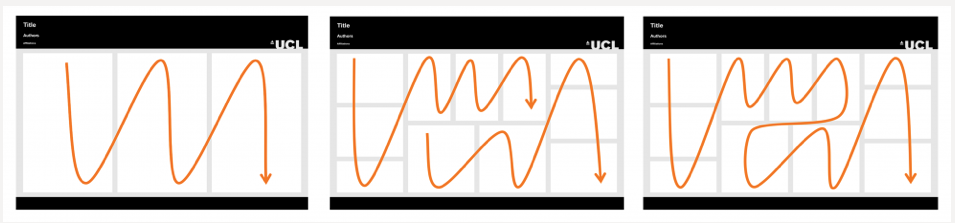
\includegraphics[keepaspectratio]{how_to_poster_files/reading_direction.png}}
\caption{(from UCL resource)}
\end{figure}

\subsubsection{Text}\label{text}

\begin{itemize}
\tightlist
\item
  Bite-size pieces of information are easier to digest than large
  chunks!
\item
  Use bigger text than you think you should!
\item
  Consider organising the text of your poster into bullets,
\item
  highlighting words that you want to \textbf{jump} off the page,
\item
  and removing 90\% of all jargon!

  \begin{itemize}
  \tightlist
  \item
    For example, \emph{I} know what the word \emph{zoonotic} means in
    the context of \emph{malaria}, but lots of people at a public
    health/applied maths/epidemiology conference may not! I'll use
    ``\emph{malaria that infects monkeys}'' instead! And, of course, a
    \emph{picture} of the zoonotic malaria transmission cycle \ldots{}
  \end{itemize}
\end{itemize}

\subsubsection{Pictures}\label{pictures}

There are lots of details that are important to a figure when we include
it in a paper, that we should subtract when we use the same information
in a slide deck or research poster. Supply the minimal detail to
understand the idea/result that your figure is communicating. Make text
big and concise and avoid technical language that we would need to read
your paper to understand. Consider colourblind-friendly colour palettes
(\href{https://colorbrewer2.org/\#type=sequential&scheme=BuGn&n=3}{these}
\href{https://colororacle.org}{resources} might be helpful).

The University of Liverpool resource has a great example of how to
format graphs for a poster:

\begin{figure}
\centering
\pandocbounded{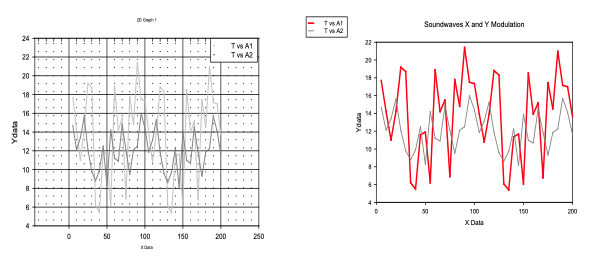
\includegraphics[keepaspectratio]{how_to_poster_files/graphs.png}}
\caption{(from University of Liverpool resource)}
\end{figure}

Another example - here's a figure I put in
\href{https://doi.org/10.1098/rsos.230641}{this paper}:

\pandocbounded{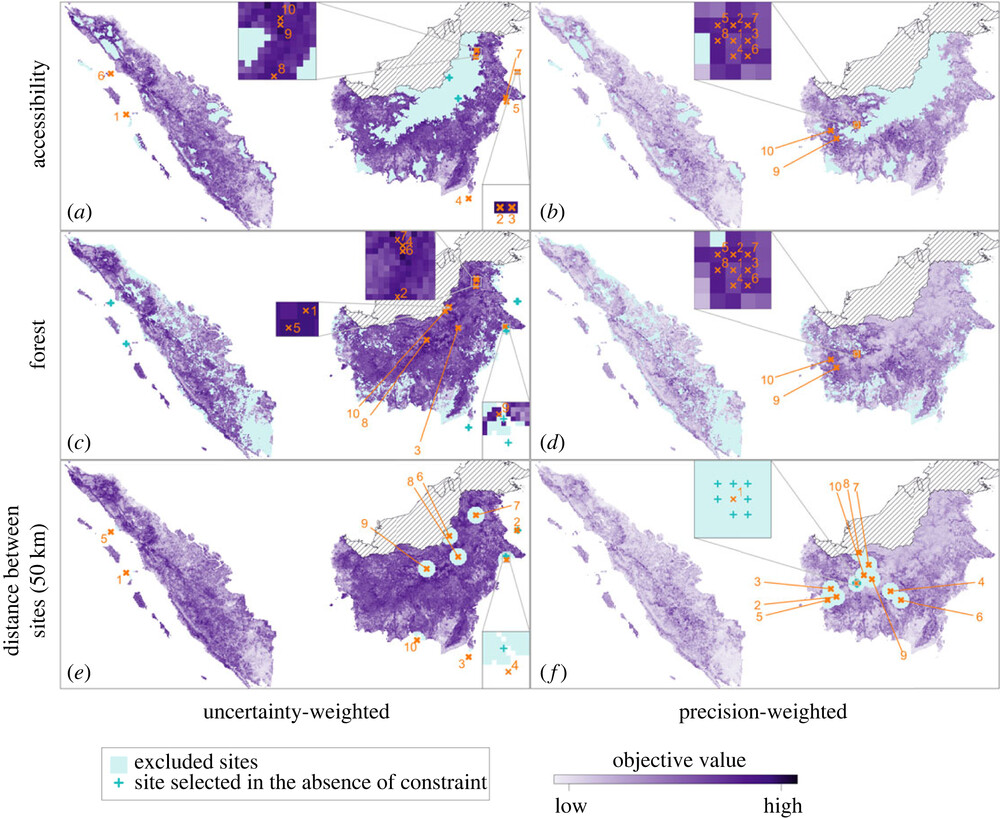
\includegraphics[keepaspectratio]{how_to_poster_files/rsos230641f04.jpg}}

\ldots{} and here's what the same information looked like when I
presented the project as a poster:

\pandocbounded{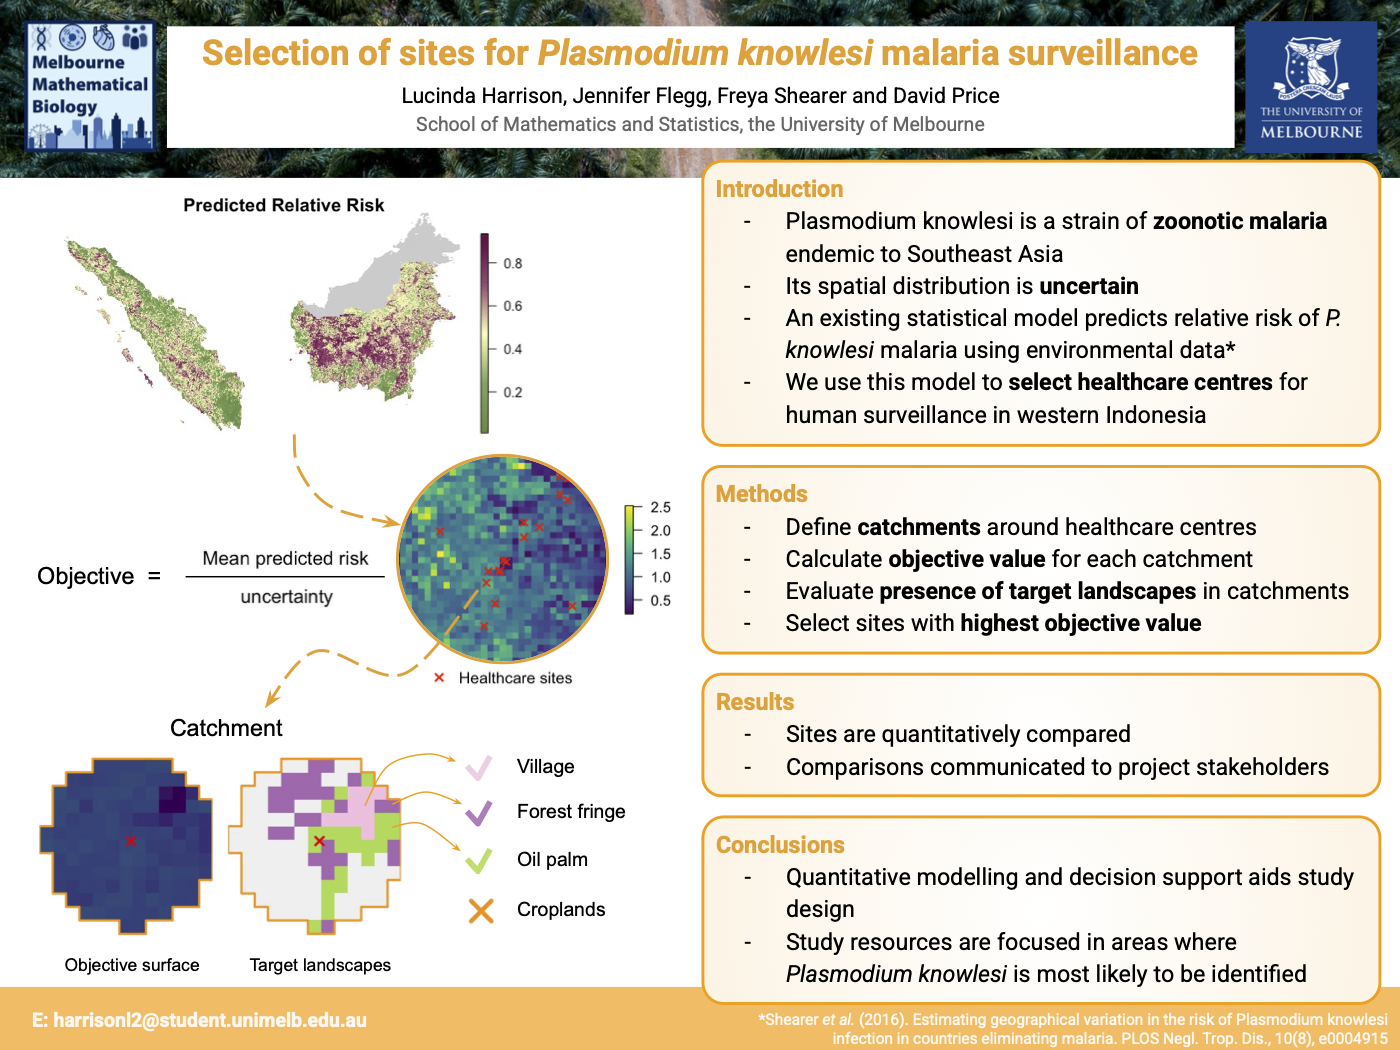
\includegraphics[keepaspectratio]{how_to_poster_files/MiM_poster.png}}

(This poster was for an online conference!)

\subsubsection{Interactive elements}\label{interactive-elements}

During a poster presentation, you only have a short window to catch the
attention of your audience. You also have an advantage over giving an
oral presentation: your audience can get right up close with your
presentation! Interactive elements to a poster presentation can really
increase audience engagement, and they don't need to be direct or
obvious. My favourite poster presentations have involved \textbf{chalk
annotations} over a mathematical model diagram, a \textbf{spring
attached to a poster} to explain the forces involved between cells in a
mathematical model of wound-healing, and a \textbf{jar of sand} to start
a discussion about the dynamics of a landslide. I presented a
\href{https://lucyharrison.shinyapps.io/pf_drug_resistance_shiny/}{Shiny
app} as a poster with fishing wire to animate buttons and sliders!

\subsection{Miscellaneous tips}\label{miscellaneous-tips}

\begin{itemize}
\item
  Don't forget to acknowledge co-authors/research groups/sponsors/grants
  involved in supporting your work (e.g., with a logo for a
  grant/sponsor)
\item
  Include a QR code to your website/linkedIn/preprint - if your audience
  has bookmarked you, they're more likely to remember your research at a
  later date!
\item
  Once you have a draft, \textbf{stand back!} Imagine your draft at A0
  size, across the other end of Radcliffe square - what things in your
  poster stand out from far away? Does it send a clear message when a
  reader can only see the title, pictures, and maybe some sub-headings?
\end{itemize}

\subsection{Some examples}\label{some-examples}

Now let's have a look at some example posters from me + my friends :)

Let's discuss:

\begin{itemize}
\tightlist
\item
  Who is the audience of each of these posters?
\item
  What do we think the poster is about when we look at it from a
  distance?
\item
  How much reading time do we need to get the gist of the poster?
\item
  What do these posters do well?
\item
  Where could these posters improve?
\end{itemize}

\subsection{Conclusion}\label{conclusion}

Hopefully now you're feeling confident and ready to whip up a great
poster!

UniOxford has a \href{https://estates.admin.ox.ac.uk/print-studio}{print
studio} which I think is available to students and staff!

\end{document}
